\chapter{\IfLanguageName{dutch}{Stand van zaken}{State of the art}}
\label{ch:stand-van-zaken}

% Tip: Begin elk hoofdstuk met een paragraaf inleiding die beschrijft hoe
% dit hoofdstuk past binnen het geheel van de bachelorproef. Geef in het
% bijzonder aan wat de link is met het vorige en volgende hoofdstuk.

% Pas na deze inleidende paragraaf komt de eerste sectiehoofding.

Gebruik van technologie:

Tegenwoordig wordt JavaScript nog heel vaak gebruikt. In maart 2019 stond JavaScript nog op de zevende plaats in de TIOBE Programming Community index\footnote{https://www.tiobe.com/tiobe-index/}. In deze index worden de meest opgezochte programmeertalen weergegeven volgens het aantal zoekopdrachten waarin deze talen voorkomen in de populairste zoekmachines ter wereld zoals Google, Yahoo! en Youtube. Tiobe Software BV is een bedrijf gevestigd in Eindhoven, Nederland dat al sinds 2001 algoritmes ontwikkelt die zich baseren op deze talloze zoekopdrachten en op basis van de resultaten de populairste programmeertalen beschrijft. \autocite{Redondo2017}

Angular of React daarentegen zijn geen talen, maar een JavaScript framework en een JavaScript library respectievelijk. Het Angular framework maakt gebruik van TypeScript, een getypeerde taal waarbij je dus bij variabelen het type moet definiëren. Aan de andere kant, gebruikt React gewoon JavaScript. Hier wordt dieper op ingegaan in xx. Vergeleken met elkaar is React altijd meer gebruikt geweest dan Angular. Figuur \ref{fig:a} toont de trend in npm downloads tussen deze twee technologieën. \autocite{Hamedani2018}
	\begin{figure}
		\centering
		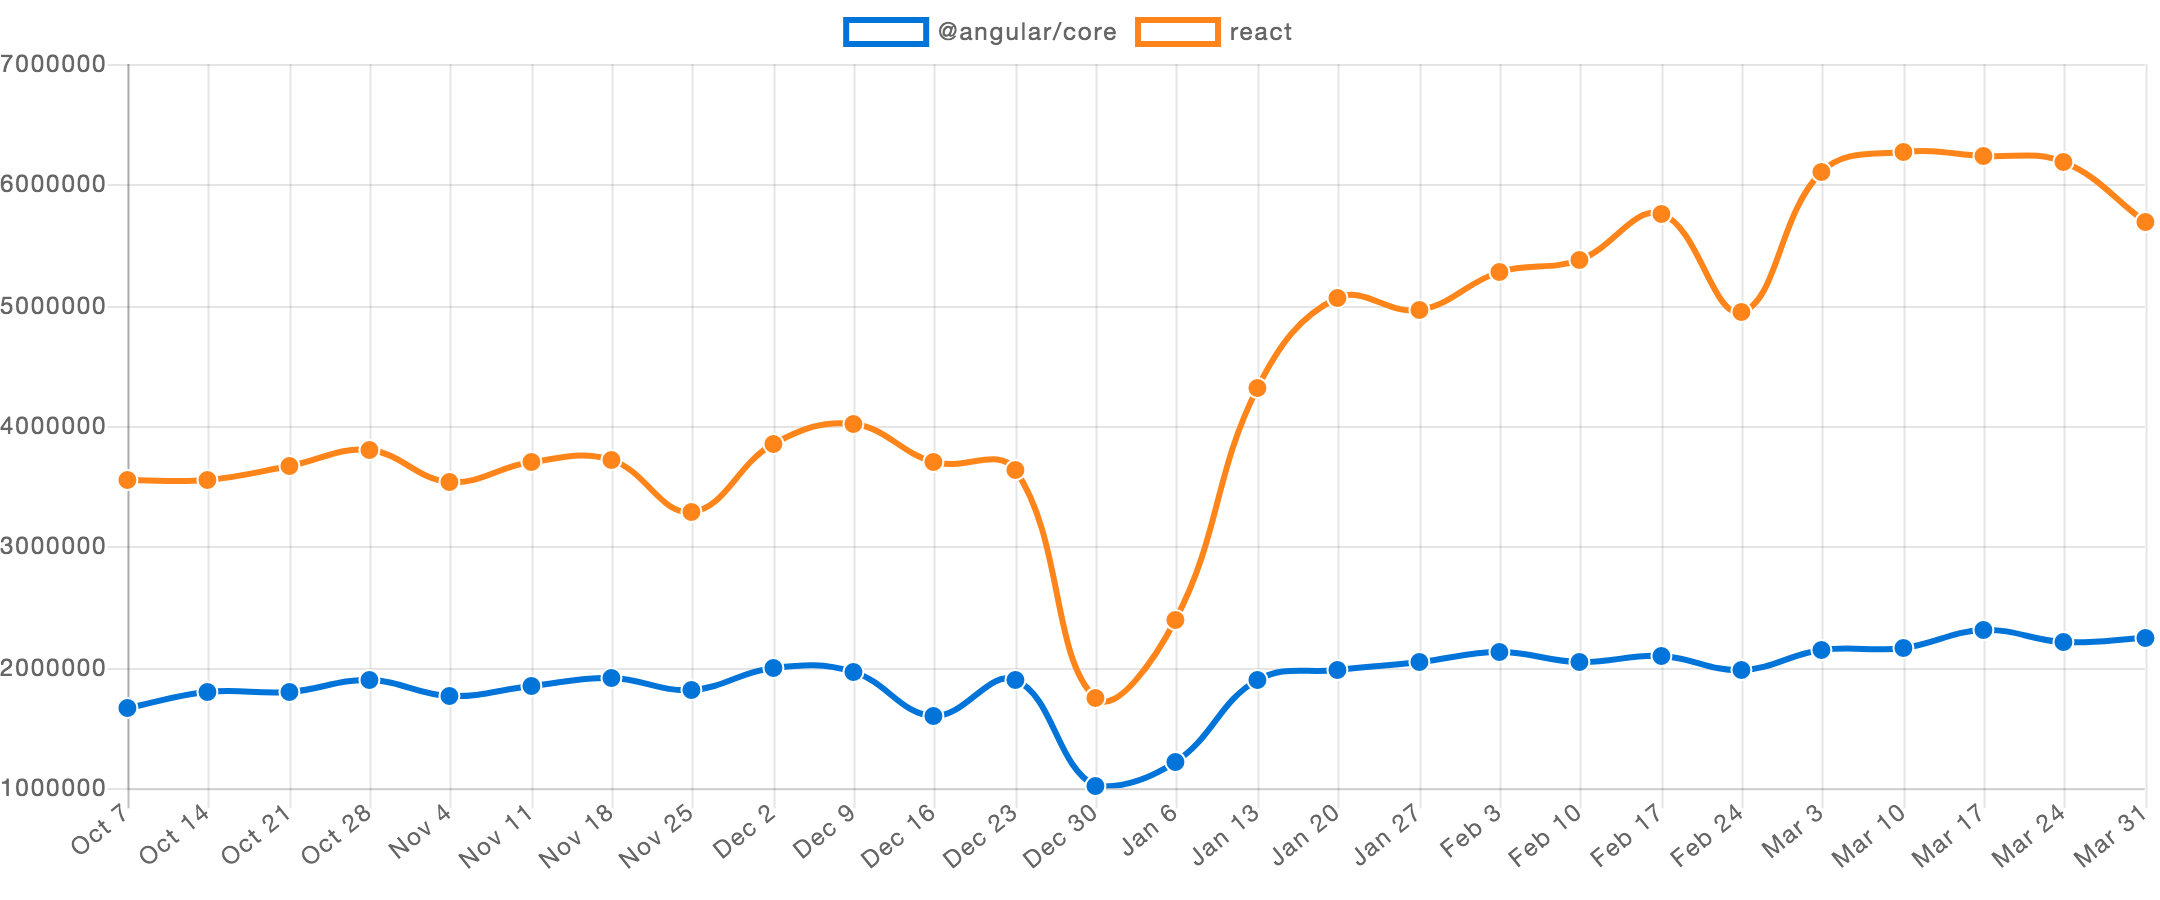
\includegraphics[width=0.75\columnwidth]{/Users/jelle/bachproef-latex-sjabloon/bachproef/npmtrends.png}
		\caption{Aantal downloads van Angular in vergelijking met React via npm in de afgelopen 6 maanden. Deze statistieken zijn te vinden op de website van npmtrends.\protect\footnotemark. }
		\label{fig:a}
	\end{figure}
\footnotetext{https://www.npmtrends.com/}

Javascript:

JavaScript is een programmeer- of scripttaal die gebruik maakt van zogenoemde 'first-class functions'. Dat wil zeggen dat functies in JavaScript verwerkt worden als een gewone variabele. Zo'n functie kan dus, met andere woorden, als argument meegegeven of geretourneerd worden en kan in een variabele opgeslagen worden. JavaScript is welgekend om zijn toepassingen in webapplicaties, maar het wordt ook gebruikt in andere omgevingen zoals Adobe Acrobat en Node.js. \autocite{Alexiou2017}

JavaScript wordt 'Just-In-Time' gecompileerd. Deze JIT compilatie zorgt ervoor dat JavaScript sneller runt door de code die uitgevoerd wordt te bekijken en veel gebruikte code paden geoptimaliseerd wordt. Dit zorgt voor een veelvoudig performantere uitvoering van JavaScript. \autocite{Clark2017}

In Adobe Acrobat\footnote{https://www.adobe.com/devnet/acrobat/javascript.html} kan JavaScript gebruikt worden om gemakkelijk PDF-bestand aan te passen. Het staat toe om objecten, methoden en eigenschappen te implementeren waarmee de bestanden aangepast kunnen worden. Node.js\footnote{https://nodejs.org/en/} maakt gebruik van Chrome's V8 JavaScript engine en staat developers toe om servergebaseerde en netwerkapplicaties te maken.

Geschiedenis van JavaScript:

De ontwikkelaars van de Netscape browser, Netscape Communications, wilden een taal ontwikkelen die webpagina's dynamischer kon maken. Dus begon de ontwikkeling Mocha, een simpele en dynamische scripttaal die leek op Java. In mei 1995 werd Mocha geïntegreerd in de Netscape browser. Kort daarna ging Mocha door twee naamsveranderingen. Eerst werd het gewijzigd naar LiveScript en uiteindelijk, in december 1995, werd de naam 'JavaScript' bedacht. Het idee hierachter was dat JavaScript bedoeld was voor kleine taken in de browser, terwijl Java eerder bedoeld was voor professionele ontwikkelaars om webcomponenten te maken. \autocite{Peyrott2017}

De eerste grote doorslag van JavaScript kwam er toen ECMA besloot om een normalisering te maken van JavaScript. ECMA is een brancheorganisatie en hun doel is om informatie en communicatietechnologieën te normaliseren. In juni 1997 werd de eerste officiële versie uitgebracht als ECMA-262. Deze normalisatie was belangrijk, want het opende JavaScript naar het publiek, waardoor meer mensen in contact kwamen met de scripttaal. Omwille van handelsmerkredenen kon ECMA de naam JavaScript niet gebruiken. Na overleg werd besloten om de normalisatie ECMAScript te noemen. JavaScript is tegenwoordig de commerciële naam van ECMAScript.\autocite{Peyrott2017}

Werking van JavaScript:

Zoals eerder vermeld, maakt JavaScript gebruik van JIT-copilatie. Wanneer een browser een webpagina wilt laden, zal de HTML-parser eerst de HTML-code parsen en het Document Object Model (DOM) maken. Als de HTML-parser op CSS of JavaScript directives stuit, zowel inline als extern geladen, zal de parser deze code doorsturen naar de CSS-parser of de JavaScript machine respectievelijk. De JavaScript machine laadt interne code en externe JavaScript bestanden, maar wacht met het uitvoeren ervan tot beide parsers klaar zijn. Hierna wordt de JavaScript code uitgevoerd in de volgorde waarop ze voorkomen in de webpagina. Deze code kan ervoor zorgen dat het DOM geüpdated wordt, deze wijzigingen zullen onmiddelijk zichtbaar zijn. https://www.makeuseof.com/tag/what-is-javascript/

Angular:

In de documentatie op de website van Angular\footnote{https://angular.io/docs} wordt volgende definitie vermeldt: Angular is een platform dat het gemakkelijk maakt om webapplicaties te bouwen. Angular combineert templates, dependency injectie, end to end tooling en geïntegreerde best practices om hindernissen in de ontwikkeling op te lossen. Angular stelt ontwikkelaars in staat om applicaties te maken voor op het web, mobiel of desktop.

Angular kan gezien worden als een volwaardig MVC\footnote{Model View Controller} framework. Het wordt zo beschouwd omdat Angular de structuur van de applicatie in ontwikkeling sterk wilt regulieren. Angular voorziet standaard veel functionaliteit. Aan de andere kant zorgt dit wel voor minder flexibiliteit. Angular verstrekt instantaan volgende functionaliteit:
\begin{itemize}
	\item Templates
	\item XSS\footnote{Cross-Site Scripting} bescherming
	\item Dependency Injectie
	\item Component CSS encapsulatie
	\item Hulpmiddelen voor het unit-testen van componenten
	\item Ajax requests
	\item Routering
	\item Formulieren
\end{itemize}

React, aan de andere kant, is een library met als doel ontwikkelaars te helpen met het bouwen van User Interfaces. De structuur van deze UI's worden voorgesteld als een boom waarbij de knopen componenten zijn. Een component bestaat uit zowel HTML als JavaScript die de logica beschrijft om deze te tonen. \autocite{Baer2018}

Elke component is eigenlijk een JavaScript functie. Deze retourneert code, deze code stelt de visuele representatie van de component voor. Deze code is wordt vertaald naar een taal genoemd JSX. JSX lijkt op HTML maar deze werkt binnen JavaScript, wat HTML niet doet. De functies worden in een bepaalde volgorde aangeroepen, waarop het resultaat dan samengevoegd wordt en getoond wordt aan de gebruiker. Op deze manier wordt een pagina gebouwd met React.  \autocite{Domes2017}






Dit hoofdstuk bevat je literatuurstudie. De inhoud gaat verder op de inleiding, maar zal het onderwerp van de bachelorproef *diepgaand* uitspitten. De bedoeling is dat de lezer na lezing van dit hoofdstuk helemaal op de hoogte is van de huidige stand van zaken (state-of-the-art) in het onderzoeksdomein. Iemand die niet vertrouwd is met het onderwerp, weet nu voldoende om de rest van het verhaal te kunnen volgen, zonder dat die er nog andere informatie moet over opzoeken \autocite{Pollefliet2011}.

Je verwijst bij elke bewering die je doet, vakterm die je introduceert, enz. naar je bronnen. In \LaTeX{} kan dat met het commando \texttt{$\backslash${textcite\{\}}} of \texttt{$\backslash${autocite\{\}}}. Als argument van het commando geef je de ``sleutel'' van een ``record'' in een bibliografische databank in het Bib\LaTeX{}-formaat (een tekstbestand). Als je expliciet naar de auteur verwijst in de zin, gebruik je \texttt{$\backslash${}textcite\{\}}.
Soms wil je de auteur niet expliciet vernoemen, dan gebruik je \texttt{$\backslash${}autocite\{\}}. In de volgende paragraaf een voorbeeld van elk.


\lipsum[7-20]
